\chapter{Onemocnění sítnice lidského oka}
\label{ch:nemoci}

\section{Věkem podmíněná makulární degenerace}
Věkem podmíněná makulární degenerace (dále jen VPMD) je onemocnění makuly, které se objevuje u~pacientů starších 50 let a je nejčastější příčinou praktické slepoty v~ekonomicky vyspělých zemích. S~rostoucím počtem seniorů se stává velkým celospolečenským zdravotním problémem. Na vznik a rozvoj tohoto onemocnění má vliv více faktorů. Kromě rostoucího věku to může být i vysoký krevní tlak, kouření, špatné stravovací návyky a s~tím spojená obezita a genetické dispozice. Pacienti popisují její projevy tak, že zraková ostrost postupně klesá, stěžují si na deformace obrazu a v~pokročilejších případech se v~centru zorného pole objevuje rozmazaná nebo někdy až černá skvrna. Rovněž dochází ke zhoršení barevného vidění. Léčitelná je jeho vlhká forma, kdy současná medicína dokáže pouze mírně zpomalit její projevy. Ke zlepšení zraku již nedojde a pouze se stabilizuje aktuální kvalita vidění \cite{Atlas}.

\subsection*{Formy věkem podmíněné makulární degenerace}
VPMD rozdělujeme na 2 formy: suchou (atrofickou, nonexsudativní) a vlhkou (exsudativní). Suchou formou je postiženo až 90 \% pacientů, ale jen u~12--21 \% způsobuje závažnou poruchu zraku. Vlhkou formou trpí méně pacientů, ale je daleko závažnější než suchá forma, protože postupuje velmi rychle. Obě dvě formy se mohou v~průběhu onemocnění kombinovat. V~makulární krajině nemocných nacházíme změny a úbytek retinálního pigmentového epitelu a drúzy. Drúzy dělíme podle vzhledu a velikosti na tvrdé a měkké. Jejich porovnání lze vidět na obrázcích \ref{pic:chap03_drusen_hard} a \ref{pic:chap03_drusen_soft}. Tvrdé drúzy jsou malá ohraničená depozita žlutavé barvy. Naopak měkké drúzy nemají ostré ohraničení a mohou i splývat, jsou spojeny s~podstatně vyšším rizikem vzniku vlhké formy VPMD. Další možnou úlohu při tvorbě drúz hrají lipidy, které se ukládají v~Bruchově membráně a brání výměně živin \cite{vpmd_kolar}.

\begin{figure}[h]
  \begin{minipage}[c]{0.47\textwidth}
    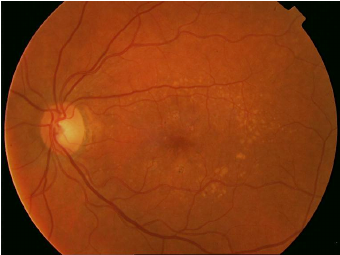
\includegraphics[width=\linewidth]{chap03_drusen_hard}
    \caption{Tvrdé drúzy \cite{vpmd_kolar}.}
    \label{pic:chap03_drusen_hard}
  \end{minipage}
  \hfill
  \begin{minipage}[c]{0.47\textwidth}
    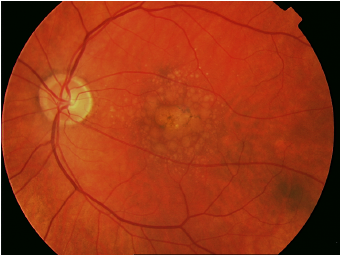
\includegraphics[width=\linewidth]{chap03_drusen_soft}
    \caption{Měkké drúzy \cite{vpmd_kolar}.}
    \label{pic:chap03_drusen_soft}
  \end{minipage}
\end{figure}


\begin{itemize}
  \item\textbf{Suchá forma} se často projevuje velmi pomalým postupným zhoršováním ostrosti vidění v~průběhu let. Včasná fáze začíná poškozením pigmentové vrstvy sítnice, která zabezpečuje metabolizmus sítnice, následně hromadění odpadních látek ve formě drúz a projevem určitého stupně atrofie. Mezi první příznaky patří rozmazané vidění, zhoršené vidění za tmy či za soumraku, zhoršení možnosti čtení nebo zaostření na jeden objekt. Geografická atrofie představuje rozvinuté stadium suché formy VPMD. Vidět ji můžete na obrázku \ref{pic:chap03_geo_atrof}. K~příznakům raného stádia patří měkké drúzy, hypopigmentace spojená s~drúzami a hyperpigmentace spojená s~drúzami. Léčba suché formy VPMD v~současné době není k~dispozici. Avšak na zastavení nebo zpomalení její progrese může mít příznivý vliv doplnění antioxidačních vitamínů C, E a minerálů zinek, selen a esenciálními omega-3 nenasycenými mastnými kyselinami. Podpůrnou úlohu má i strava bohatá na ryby, listovou zeleninu a ovoce \cite{vpmd_kolar}.
  
  \begin{figure}[h]
    \begin{center}
      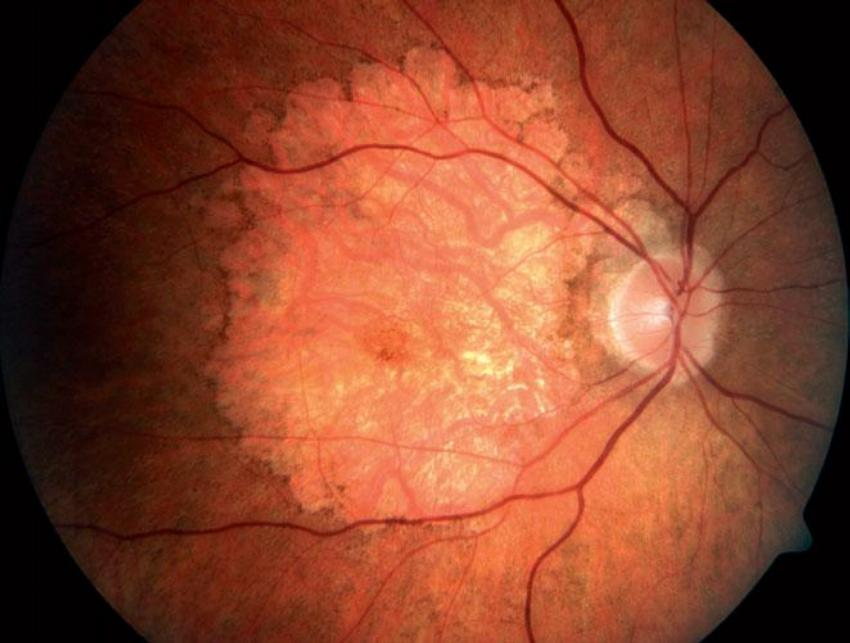
\includegraphics[width=.6\linewidth]{chap03_geo_atrof}
      \caption{Geografická atrofie \cite{pic_geo_atrof}.}
      \label{pic:chap03_geo_atrof}
    \end{center}
  \end{figure}

  \item\textbf{Vlhká forma} v~porovnání se suchou formou postupuje rychleji a ztráta vidění je výraznější. K~rapidnímu zhoršení dochází v~průběhu několika týdnů a k~praktické slepotě již během pár měsíců. Je způsobena podrůstáním nových cév pod sítnici, které postupně začínají prosakovat, a tím způsobí otok nebo krvácení. Prosakování a krvácení stimuluje tvorbu vazivové tkáně a v~makule se vytvoří útvar, který se nazývá pseudotumor. Základními projevy onemocnění jsou deformace vnímaného obrazu, výpadek zejména centrální části zorného pole, pokles centrální zrakové ostrosti hůře vnímaný do blízka a charakteristický nález na očním pozadí (viz obrázek \ref{pic:chap03_soft_armd}). Onemocnění vede k~úplné ztrátě centrálního vidění, periferní vidění je zachováno. Léčba dříve spočívala v~destrukci neovaskulární membrány fotokoagulačním nebo termoterapeutickým laserem. Výsledky léčby však byly kolísavé. Východiskem měla být cílenější tzv. fotodynamická terapie, při které je nitrožilně podaná látka absorbována cílovou tkání a poté aktivována laserem \cite{vpmd_kolar}.
  
  \begin{figure}[h]
    \begin{center}
      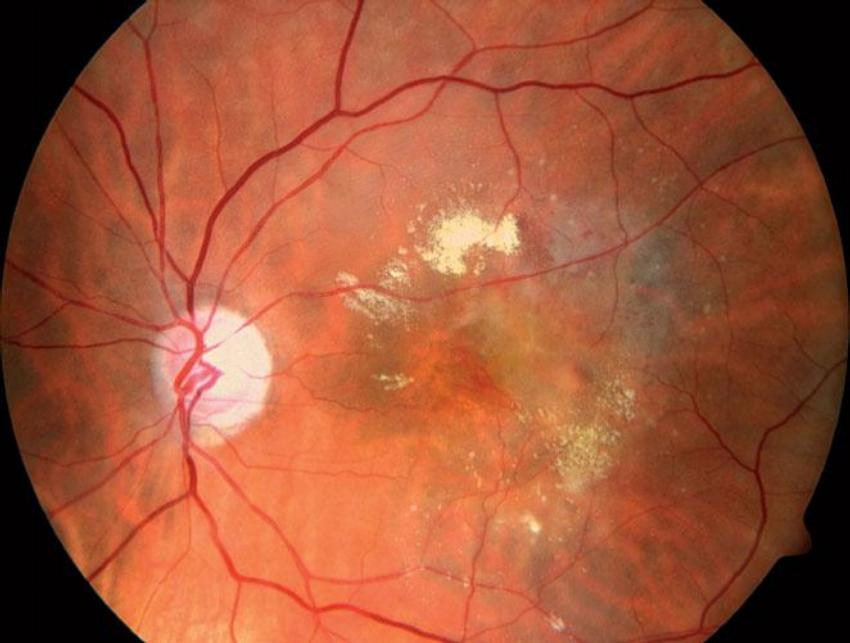
\includegraphics[width=0.6\linewidth]{chap03_soft_armd}
      \caption{Vlhká forma s~edémem \cite{pic_soft_armd}.}
      \label{pic:chap03_soft_armd}
    \end{center}
  \end{figure}

\end{itemize}


\section{Retinopatie}
V~souvislosti s~celkovými onemocněními, jako je vysoký krevní tlak nebo arterioskleróza, se mohou rozvíjet trvalé změny na sítnici, které nazýváme retinopatie. Dochází postupně ke zužování cév a poklesu krevního zásobení sítnice až k~postižení zrakového nervu a nevratným změnám.  

Zvláštním případem retinopatie je retinopatie diabetická. Projeví se asi po 8--10 letech trvání cukrovky. Pacient zaznamenává výpadky zorného pole nebo pokles zrakové ostrosti. Na tento typ onemocnění navazuje celá řada komplikací jako je zánět duhovky, šedý zákal, zánět nervů apod. Předpokladem úspěšné léčby diabetického poškození sítnice je především stabilizace cukrovky. Velmi často dochází k~degeneraci sítnice, což zahrnuje nezánětlivé změny na sítnici, které jsou spojeny s~poškozením nervových buněk. Vznikají na dědičném základě a postihují obvykle obě oči současně \cite{nemoci}.


\section{Odchlípení sítnice}
Jedná se o~velmi vážné onemocnění, které může postihnout člověka v~jakémkoliv věku, nejčastěji jsou tímto onemocněním postiženi jedinci středního a staršího věku. Projevuje se záblesky před očima, drobnými tečkami či tmavým stínem v~zorném poli. K~odchlípení sítnice oka dochází, když se v~sítnici objevují různé trhlinky, které způsobují, že tekutina ze sklivce se začne dostávat pod sítnici a nadzvedávat ji (tím se sítnice odlučuje od vrstvy pigmentových buněk). Díky tomu se pak do sítnice nedostávají živiny a kyslík, a proto buňky přítomné v~sítnici rychle odumírají. Nejčastěji k~tomuto odchlípnutí dochází na okraji sítnice, odtud se ale při neléčení pomalu přesouvá i do centra vidění. V~některých případech odchlípnutí sítnice způsobilo i svrašťování sklivce, k~němuž běžně dochází v~rámci stárnutí člověka. Při stárnutí (někdy i při úrazu, nebo krátkozrakosti či zánětu) vznikají v~sítnici drobná ložiska, která mohou vytvářet nové spojení mezi sklivcem a sítnicí. Právě tato spojení způsobují, že může dojít k~vytržení části sítnicové tkáně, když se sklivec smršťuje. 

Pokud lékař objeví trhliny nebo díry v~sítnici ještě před vznikem odchlípnutí, využívá se laserová koagulace, kterou se sítnice připojí k~ostatním vrstvám oční stěny. Pokud již ale k~odchlípnutí sítnice došlo, jediným řešením je operace pod celkovou anestezií \cite{nemoci}.  


\section{Prasklá sítnice}
Sítnice může v~oku člověka prasknout z~různých důvodů. Může to být důsledek komplikací jiného očního onemocnění, může se jednat o~degenerativní formu onemocnění očí nebo k~tomu může dojít také při poranění očí či mozku. K~tomuto prasknutí dochází obvykle v~důsledku toho, že sítnice není delší dobu správně prokrvována. Vliv na prasknutí může mít i stáří oční bulvy.
Pokud se jedná o~drobné prasklinky v~sítnici, tak si pacient nemusí uvědomovat žádné problémy se zrakem, ale i přesto na sobě může postupně vypozorovat různé příznaky jako světlé záblesky před očima, zužování viditelného pole a další. Pokud je ale sítnice oka porušená výrazněji může dojít k~výraznému zhoršování zraku, i k~jeho ztrátě.

Léčba praskliny může probíhat pomocí laseru, kryoterapií i chirurgickým zákrokem. O~formě léčbu rozhoduje vždy lékař v~závislosti na rozsahu, typu a umístění praskliny.


\section{Zánět sítnice}
Toto onemocnění je také známé pod označení retinitida. Projevuje se rozmazaným viděním a pohyblivými skvrnami v~zorném poli. Typická je také vysoká citlivost na světlo a slzení. Zánět sítnice oka mohou způsobit viry i paraziti, nejčastější příčinou jsou ale bakterie. Pacientovi se infekce do sítnice může dostat krví ze zánětlivého ložiska v~podstatě kdekoliv v~těle. Sítnice se může zanítit i po úrazu nebo v~případě, kdy je infekce do oka zanesena přímo (například promnutí oka rukou). Když tělo léčí tuto infekci, tak imunitní buňky poškozují současně i buňky v~sítnici, což může vést ke zhoršování zraku. V~mnoha případech není zánět sítnice osamocený a doprovází ho také zánět cévnatky, která sítnici zásobí krví.

K~léčbě zánětu sítnice oka obvykle lékař předepíše antibiotika, v~závažnějších případech může předepsat i kortikoidy. Obvykle záleží na tom, co zánět způsobilo. Antibiotika se samozřejmě nepředepisují v~případě, že onemocnění způsobily viry, v~takovém případě se nasazují antivirotika.


\section{Otok sítnice}
Otok sítnice neboli diabetický makulární edém postihuje, jak již název napovídá, diabetiky. K~tomuto otoku dochází po prosáknutí makuly tekutinou. Otok sítnice způsobuje, že se snižuje schopnost vnímat světlo. Díky tomu  má pacient rozmazané vidění a není schopen zaostřit oko. Tento otok se může objevit u~lidí, kteří cukrovkou trpí dlouhodobě, nebo pokud i při léčbě mají příliš vysokou hladinu glukózy. Otok je způsoben poškozením cév v~sítnici a jejím okolí. Tyto cévky pak propouštějí tekutinu do sítnice, kde se hromadí, a tím vzniká otok.

Pokud by nedošlo k~léčbě, může otok sítnice vést až k~úplné ztrátě zraku. Léčba otoku sítnice musí probíhat v~závislosti na léčbě cukrovky,  kdy se hladina cukru v~krvi udržuje ve vhodných hodnotách. Otok sítnice se obvykle léčí laserovou operací očí, kdy se laserem spálí prosakující cévy, a tím se uzavřou.


\section{Oběhové poruchy sítnice}
Poměrně častým onemocněním sítnice jsou oběhové poruchy, kdy dochází k~uzávěru sítnicových cév. Tyto uzávěry vznikají většinou jako důsledek arteriosklerózy, což je degenerativní onemocnění cév, kde dochází k~jejím zužování a k~horšímu krevnímu zásobení tkání. Vznik arteriosklerózy je podporován některými celkovými chorobami jako je vysoký krevní tlak, cukrovka, porucha metabolismu tuků apod \cite{nemoci}.

Při \textbf{uzávěru centrální sítnicové tepny} dochází k~náhlému zhoršení vidění. Na očním pozadí je vidět zúžená tepna, dochází k~nedokrvení a otoku sítnice. Je důležité, aby byla léčba zahájena včas, nejlépe do dvou hodin od vzniku prvních příznaků. Aplikují se léky na rozšíření cév, léky na rozpuštění trombu a léky zabraňující srážení krve. I~přes včasnou léčbu bývá funkce sítnice často snížena.

\textbf{Uzávěr centrální sítnicové žíly} se projevuje rychlým zhoršováním vidění, trombus způsobuje přetlak žíly, rozšíření žíly je nepravidelné a dochází ke krvácení do sítnice. Podávají se léky na rozšíření cév, po čase se tromby vstřebávají, popřípadě se pomocí laseru zlepšují oběhové poměry v~sítnici.
